\chapter{Музыкальные композиции}
\label{ch:musical-composition}
Глава посвящена исследованию музыкальных композиций на основе Викиданных. С помощью SPARQL-запросов, вычисляемых на объектах типа <<музыкальная композиция>> в~Викиданных получены списки: всех музыкальных композиций, музыкальных композиций, имеющих композиторов, музыкальных композиций, объединённых по жанрам и по годам, также построена пузырьковая диаграмма, показывающая композиторов с наибольшим количеством композиций. Найден список музыкальных произведений в Викиданных, для которых будет законно зарузить их аудиозапись на Викисклад, поскольку истек их копирайт.

\section{Число <<Музыкальных композиций>> и жанры}

\marginnote{Используемые в запросах объекты: <<\wdqName {музыкальное произведение/композиция} {105543609}>>;
используемое свойство: <<\wdProperty{31}{экземпляр}>>.}

Построим список всех музыкальных композиций с помощью запроса~\ref{lst:musical_composition}.

\begin{lstlisting}[ language=SPARQL,
                    caption={\href{https://w.wiki/85dR}{Список всех  музыкальных композиций}\protect\footnotemark},
                    label=lst:musical_composition,
                    texcl,
	         numbers=none
                    ]
# List of all musical compositions
SELECT ?composition ?compositionLabel 
WHERE {
  ?composition wdt:P31 wd:Q105543609. # instance of musical work
  SERVICE wikibase:label { bd:serviceParam wikibase:language "ru,en" }
}
\end{lstlisting}%
\footnotetext{Получено: \num{5495} записей на 2017 год и \num{150,5} тыс. записей на~2023 год. Ссылка на SPARQL-запрос: \href{https://w.wiki/85dR}{https://w.wiki/85dR}.}

Наиболее полными и проработанными примерами музыкальных композиций на Викиданных являются: <<\wdqName{Волшебная флейта}{5064}>>, <<\wdqName{К Элизе}{11980}>>, <<\wdqName{Реквием}{207875}>>, <<\wdqName{Маленькая ночная серенада}{12025}>>, <<\wdqName{Соната си синор}{63681379}>>.

В 2022 году по запросу~\ref{lst:musical_composition} найдено \num{106,7} тыс. музыкальных композиций, а в 2023~--- \num{150,5} тыс. музыкальных композиций, вместо \num{5,5} тыс. в 2017 году. Увеличение числа композиций связано с тем, что эти объекты Викиданных являются теперь не экземплярами объекта «музыкальное произведение», а экземплярами различных подклассов «музыкальное произведение». При поиске подклассов объекта «музыкальное произведение» можно найти такие жанры: <<\wdqName{песня}{7366}>>, <<\wdqName{духовная песня}{856713}>>, <<\wdqName{гимн}{484692}>>. Более подробно анализ музыкальных жанров будет представлен в разделе <<Количество музыкальных произведений по~жанрам>> на стр. 96.

Найдём количество музыкальных композиций в каждом жанре с помощью запроса~\ref{lst:music _in_each_subclass}.

\begin{lstlisting}[ language=SPARQL,
                    caption={\href{https://w.wiki/8PzR}{ Количество музыкальных композиций в каждом подклассе}\protect\footnotemark},
                    label=lst:music _in_each_subclass,
                    texcl
                    ]
# Count of pieces of music in each subclass
SELECT ?type (COUNT(?typeInstance) AS ?count) ?typeLabel WHERE {
  ?type wdt:P279* wd:Q105543609.      # subclass of musical composition
  ?typeInstance wdt:P31 ?type.  # instance  of that class of which this subject is a particular example and member
  SERVICE wikibase:label { bd:serviceParam wikibase:language "ru, en" }
}
GROUP BY ?type ?typeLabel
ORDER BY DESC (?count)
\end{lstlisting}%
\footnotetext{Получено: \num{161} подкласс музыкальных композиций на 2022 год. Ссылка на SPARQL-запрос: \href{https://w.wiki/8PzR}{https://w.wiki/8PzR}.}

Теперь подсчитаем общее суммарное число музыкальных произведений с учётом музыкальных композиций в подклассах. Для этого добавим в~запрос~\ref{lst:music _in_each_subclass} команду \lstinline|SUM()| в~строку~2 и удалим лишние строки, чтобы получить запрос~\ref{lst:The_total_number_of_musical_works_for_all_subclasses}.

\begin{lstlisting}[ language=SPARQL,
                    caption={\href{https://w.wiki/5$BT}{ Суммарное число музыкальных произведений с учётом музыкальных композиций в подклассах}\protect\footnotemark},
                    label=lst:The_total_number_of_musical_works_for_all_subclasses,
                    texcl,
	         xleftmargin=18pt
                    ]
# The total number of musical works for all subclasses 
SELECT (SUM(?count) AS ?sum) WHERE{
  SELECT (COUNT(?music) AS ?count) WHERE {
    ?type wdt:P279* wd:Q105543609.  # subclass of musical composition
    ?music wdt:P31 ?type  # instance  of that class of which this subject is a particular example and member
  }
}
\end{lstlisting}%
\footnotetext{Получено: \num{145046} музыкальных произведений на 2022 год и \num{164} тыс. на 2023 год. Ссылка на~SPARQL-запрос: \href{https://w.wiki/5$BT}{https://w.wiki/5\$BT}.}

Можно записать этот код еще короче. Переменная \lstinline|?type| нам не нужна, поэтому можно обойтись без неё, а 4 и 5 строки поменяем местами, получаем запрос~\ref{lst:The_total_number_of_musical_works_for_all_subclasses_up}.

\begin{lstlisting}[ language=SPARQL,
                    caption={\href{https://w.wiki/5$BP}{ Суммарное число музыкальных произведений с учётом музыкальных композиций в подклассах}\protect\footnotemark},
                    label=lst:The_total_number_of_musical_works_for_all_subclasses_up,
                    texcl,
	         numbers=none
                    ]
# The total number of musical works for all subclasses 
SELECT (SUM(?count) AS ?sum) WHERE{
  SELECT (COUNT(?music) AS ?count) WHERE {
    ?music wdt:P31   # instance of
          [ wdt:P279* wd:Q105543609 ]. # subclass of musical composition
  }
}
\end{lstlisting}%
\footnotetext{Получено: \num{164} тыс. музыкальных произведений на 2023 год. Ссылка на~SPARQL-запрос: \href{https://w.wiki/5$BP}{https://w.wiki/5\$BP}.}

По сравнению с 2017 годом, когда было получено \num{5494} записи, число записей увеличилось в десятки раз. Это связано с тем, что за 5 лет было добавлено множество новых музыкальных произведений, а также старых, которые не были учтены ранее.
Напишем скрипт~\ref{lst:Musical_comp_2018--2023} и посмотрим сколько новых и старых (то есть созданных до 2018 года) музыкальных произведений было добавлено в~Викиданные за~период с~2018 года по~2023 год.

\begin{lstlisting}[ language=SPARQL,
                    caption={\href{https://w.wiki/8P$N}{ Количество музыкальных композиций в период 2018--2023 годы}\protect\footnotemark},
                    label=lst:Musical_comp_2018--2023,
                    texcl,
	         xleftmargin=18pt
                    ]
# The total number of musical works for all subclasses 
SELECT (SUM(?count) AS ?sum) WHERE{
  SELECT (COUNT(?composition) AS ?count) WHERE{
    ?composition wdt:P31 wd:Q105543609;  # subclass of musical composition
     wdt:P577 ?publication.                # composition has a publication date
  BIND(YEAR(?publication) AS ?year)
  FILTER(?publication > "2018-01-01T00:00:00Z"^^xsd:dateTime)
    }
}
\end{lstlisting}%
\footnotetext{Получено: \num{3234} музыкальных произведений за 2018--2023 годы. Ссылка на SPARQ-запрос: \href{https://w.wiki/8P$N}{https://w.wiki/8P\$N}.}

За пять лет было добавлено \num{159} тыс. произведений, из них всего \num{3234} были написаны композиторами за 2018--2023 годы, что составляет 2\,\% от всех добавленных произведений. Остальные \num{156} тыс. произведений были написаны до 2018 года, а добавлены в Викиданные после 2017 года.

Сравнив результаты запросов~\ref{lst:Musical_comp_2018--2023} и~\ref{lst:The_total_number_of_musical_works_for_all_subclasses_up} мы не учли следующую проблему: если не учитывать строку 7 в запросе~\ref{lst:Musical_comp_2018--2023}, то получим \num{51} тыс. музыкальных произведений, что почти в~три раза меньше, чем \num{159} тыс. проиведений. Связано это с тем, что в запросе~\ref{lst:Musical_comp_2018--2023} мы учитываем условие <<\wdProperty{577}{дата публикации}>>, из-за чего получаем список только тех музыкальных произведений, у которых заполнено это условие. В запросе~\ref{lst:The_total_number_of_musical_works_for_all_subclasses_up} условие  <<\wdProperty{577}{дата публикации}>> не учитывается, следовательно, у музыкальных произведений в результате этого запроса~\ref{lst:The_total_number_of_musical_works_for_all_subclasses_up}, условие <<\wdProperty{577}{дата публикации}>> может быть не заполнено. Тогда будет корректно сравнить результаты запроса~\ref{lst:Musical_comp_2018--2023} со cтрокой 7 и без нее. За всё время было добавлено \num{51090} музыкальных произведений с заполненным условием <<\wdProperty{577}{дата публикации}>>, из них всего \num{3234} были написаны за 2018--2023 годы, что составляет 6,3\,\%.

\section{Количество музыкальных произведений по годам}
Посчитаем количество музыкальных произведений написанных в каждом десятилетии со второй половины XIX века до настоящего времени. Получим запрос~\ref{lst:The_number_of_musical_compositions_for_every_10_years} и рис. к нему~\ref{fig:diagram_10_years}.

\begin{lstlisting}[ language=SPARQL,
                    caption={\href{https://w.wiki/7wHy}{ Количество музыкальных композиций написанных за каждые 10 лет}\protect\footnotemark},
                    label=lst:The_number_of_musical_compositions_for_every_10_years,
                    texcl,
	         numbers=none
                    ]
# The number of musical compositions for every 10 years
#defaultView:BarChart
SELECT (STR(?date) AS ?date_str) (COUNT(?composition) AS ?count) WHERE {
  ?composition wdt:P31 wd:Q105543609;     # instance of compostion
    wdt:P86 ?composer;                    # composition has a composer
    wdt:P577 ?publication.                # composition has a publication date
  BIND(YEAR(?publication) AS ?year)
  BIND((FLOOR(?year / 10 )) * 10  AS ?date)
  FILTER(?publication > "1850-01-01T00:00:00Z"^^xsd:dateTime)
  FILTER(?publication < "2030-01-01T00:00:00Z"^^xsd:dateTime) 
  FILTER (!wikibase:isSomeValue(?publication)) # field "date" must be filled
}
GROUP BY ?date
ORDER BY (?date)
\end{lstlisting}%
\footnotetext{Ссылка на SPARQL-запрос: \href{https://w.wiki/7wHy}{https://w.wiki/7wHy}.}

\begin{marginfigure}[0\baselineskip]
	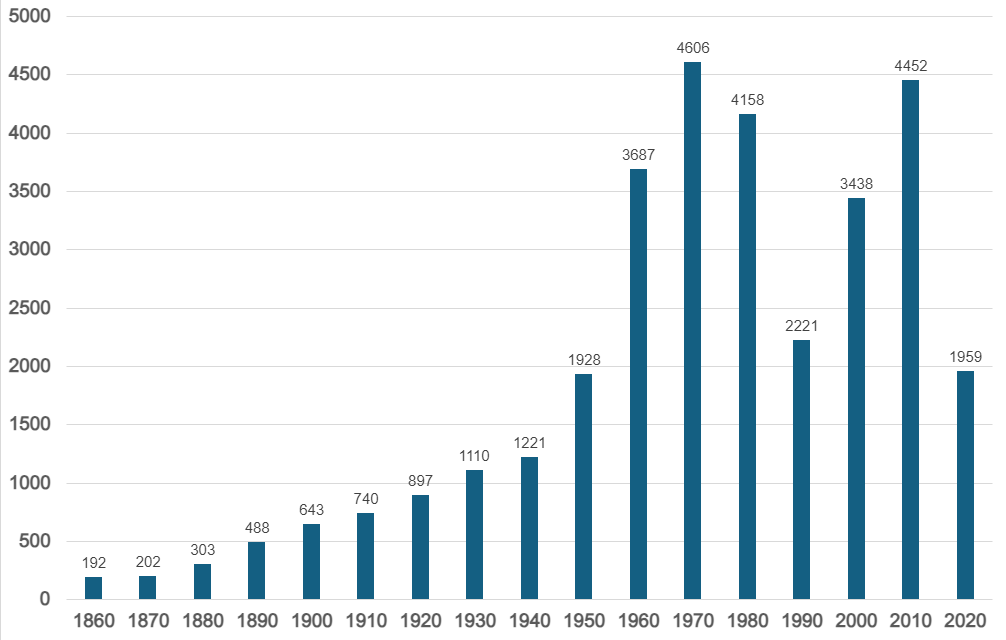
\includegraphics[width=1\textwidth]{./chapter/musical_composition/BarChart_of_The_number_of_music_compositions_for_every_10_years.svg.png}
	\caption[Гистограмма количества музыкальных композиций за каждые 10 лет с XIX века до настоящего времени]{Гистограмма количества музыкальных композиций за каждые 10 лет со второй половины XIX века до настоящего времени}%
	\label{fig:diagram_10_years}%
\end{marginfigure}
Из графика~\ref{fig:diagram_10_years} можно увидеть, что до 1890 года (1850--1890 годы) количество написанных музыкальных произведений невелико. После 1890 года (1890--1970 годы) начинается резкий подъем и продолжается до нашего времени. Такое увеличение музыкальных произведений можно объяснить тем, что со временем появляются новые жанры и новые устройства для записи. На гистограмме~\ref{fig:diagram_10_years} видим два пика: 1960-е--1980-е, 2000-е и 2010-е.


\section{Количество музыкальных произведений по жанрам}
Найдём, в каких жанрах были написаны музыкальные произведения в пиках графика~\ref{fig:diagram_10_years} и изобразим жанры на круговой диаграмме~\ref{fig:Genre_Chart_1960_—_1980} полученной по запросу~\ref{lst:count_of_pieces_of_music_in_each_subclass}. Рассмотрим первый пик: 1960-е--1980-е назовем этот пик (<<Первая волна>>).
\begin{marginfigure}[0\baselineskip]
	\includegraphics[width=1\textwidth]{./chapter/musical_composition/Genre_Chart_1960_—_1980.png}
	\caption[Круговая диаграмма музыкальных жанров за 1960--1980 годы во всем мире]{Круговая диаграмма музыкальных жанров за 1960--1980 годы во всем мире. Ссылка на SPARQL-запрос: \href{https://w.wiki/6Vx5}{https://w.wiki/6Vx5}.}%
	\label{fig:Genre_Chart_1960_—_1980}%
\end{marginfigure}
\begin{lstlisting}[ language=SPARQL,
                    caption={\href{https://w.wiki/6Vx5}{ Количество музыкальных произведений в каждом жанре}\protect\footnotemark},
                    label=lst:count_of_pieces_of_music_in_each_subclass,
                    texcl,
                    ]
# Count of pieces of music in each subclass
SELECT ?type (COUNT(?typeInstance) AS ?count) ?typeLabel WHERE {
  ?type (wdt:P279*) wd:Q207628.
  ?typeInstance wdt:P31 ?type.
  ?typeInstance wdt:P577 ?publication.
  ?typeInstance wdt:P86 ?composer.
  FILTER(?publication > "1960-01-01T00:00:00Z"^^xsd:dateTime)        
  FILTER(?publication < "1990-01-01T00:00:00Z"^^xsd:dateTime)
  SERVICE wikibase:label { bd:serviceParam wikibase:language "ru, en". }
}
GROUP BY ?type ?typeLabel
ORDER BY DESC (?count)
\end{lstlisting}%
\footnotetext{Получено: \num{27} подклассов на 2023 год. Ссылка на SPARQL-запрос: \href{https://w.wiki/6Vx5}{https://w.wiki/6Vx5}.}

Строки 7 и 8 в запросе~\ref{lst:count_of_pieces_of_music_in_each_subclass} определяют промежуток времени с 1960 года до 1990 год, который является <<первой волной>>, в этом промежутке будет производиться поиск музыкальных произведений по дате их публикации.


Теперь рассмотрим второй пик графика~\ref{fig:diagram_10_years}: 2000-е и 2010-е (<<вторая волна>>) рис.~\ref{fig:Genre_Chart_2000_—_2010}, пользуясь запросом~\ref{lst:count_of_pieces_of_music_in_each_subclass_2}.

\begin{lstlisting}[ language=SPARQL,
                    caption={\href{https://w.wiki/6Vx6}{ Количество музыкальных произведений в каждом жанре}\protect\footnotemark},
                    label=lst:count_of_pieces_of_music_in_each_subclass_2,
                    texcl 
                    ]
# Count of pieces of music in each subclass
SELECT ?type (COUNT(?typeInstance) AS ?count) ?typeLabel WHERE {
  ?type (wdt:P279*) wd:Q207628.
  ?typeInstance wdt:P31 ?type.
  ?typeInstance wdt:P577 ?publication.
  ?typeInstance wdt:P86 ?composer.
  FILTER(?publication > "2000-01-01T00:00:00Z"^^xsd:dateTime)        
  FILTER(?publication < "2020-01-01T00:00:00Z"^^xsd:dateTime)
  SERVICE wikibase:label { bd:serviceParam wikibase:language "ru, en". }
}
GROUP BY ?type ?typeLabel
ORDER BY DESC (?count)
\end{lstlisting}%
\footnotetext{Получено: \num{19} подклассов на 2023 год. Ссылка на SPARQL-запрос: \href{https://w.wiki/6Vx6}{https://w.wiki/6Vx6}.}

\begin{marginfigure}[0\baselineskip]
	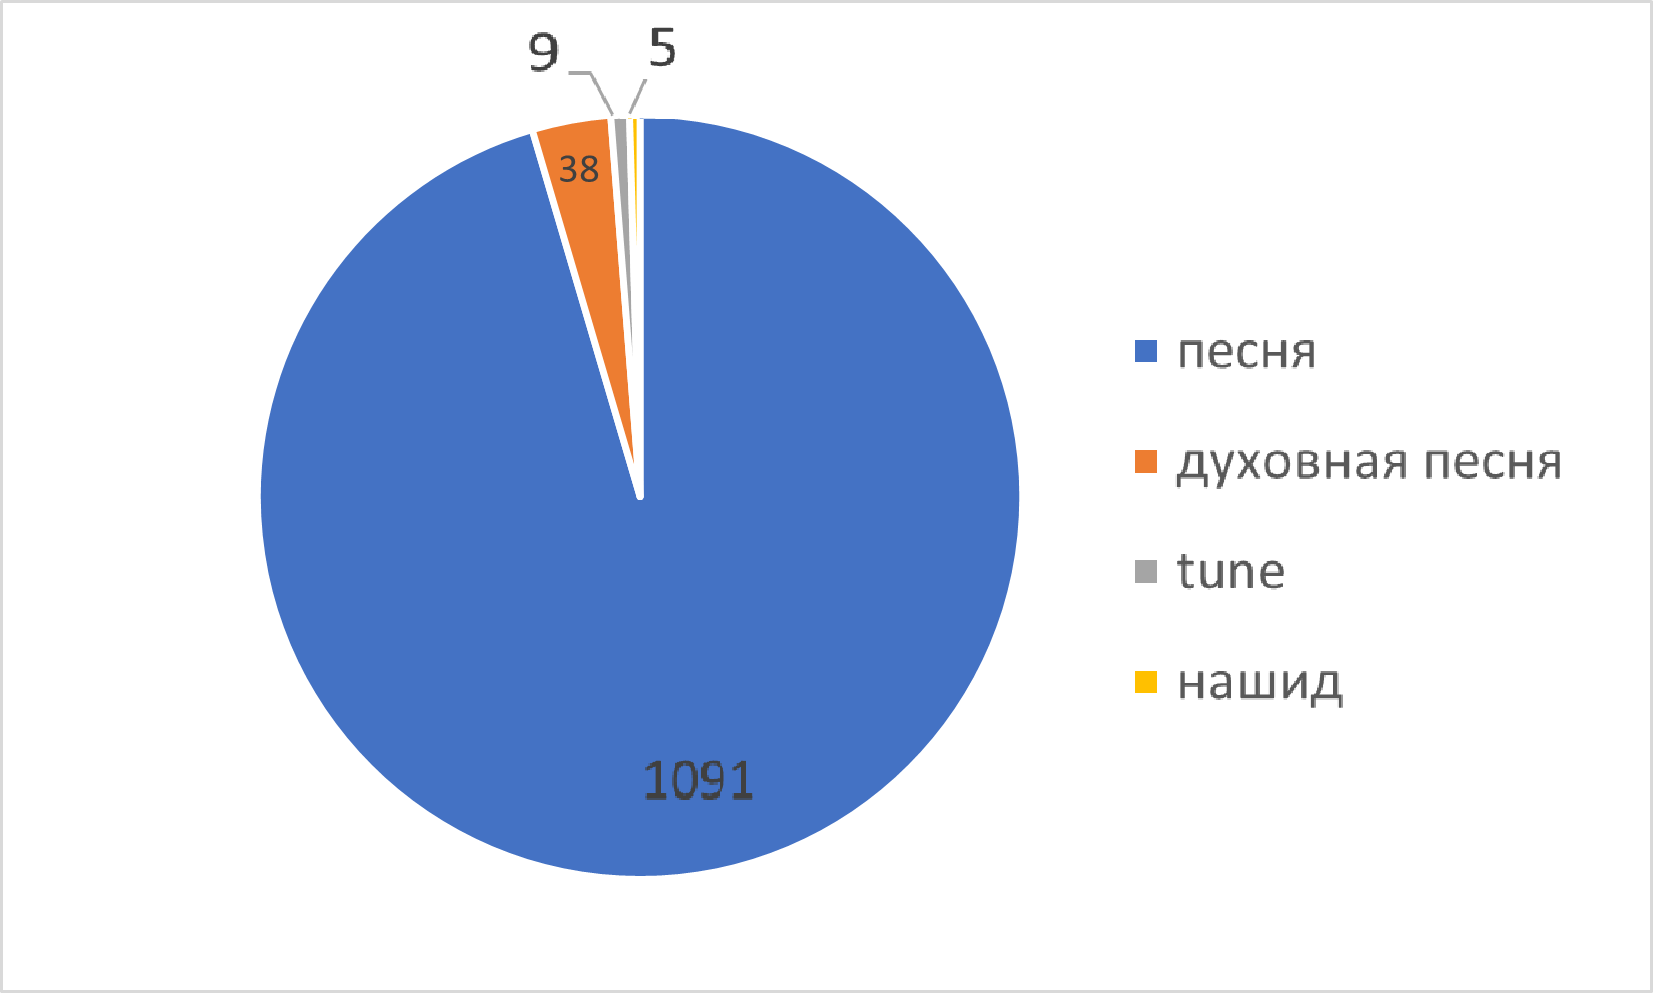
\includegraphics[width=1\textwidth]{./chapter/musical_composition/Genre_Chart_2000-2010.png}
	\caption[Круговая диаграмма музыкальных жанров за 2000--2010 годы во всем мире]{Круговая диаграмма музыкальных жанров за 2000--2010 годы во всем мире. Ссылка на SPARQL-запрос: \href{https://w.wiki/6Vx6}{https://w.wiki/6Vx6}.}%
	\label{fig:Genre_Chart_2000_—_2010}%
\end{marginfigure}

Из результатов запроса~\ref{lst:count_of_pieces_of_music_in_each_subclass} и запроса~\ref{lst:count_of_pieces_of_music_in_each_subclass_2}, можем сделать вывод, что жанры музыкальных произведений первого пика, не отличаются от жанров второго. На второй диаграмме~\ref{fig:Genre_Chart_2000_—_2010}, видим, что 95,5\,\% музыкальных произведений написаны в жанре <<песня>>. В жанре <<духовная песня>> количество музыкальных произведений по сравнению с рис.~\ref{fig:Genre_Chart_1960_—_1980} уменьшилось почти в 4 раза. А такие музыкальные жанры, как: <<переведенная песня>> и <<лирико-музыкальное произведение>> на диаграмме~\ref{fig:Genre_Chart_2000_—_2010} по сравнению с диаграммой~\ref{fig:Genre_Chart_1960_—_1980} пропали.

\section{Число композиций по десятилетиям в России}
Добавим в запрос~\ref{lst:count_of_pieces_of_music_in_each_subclass_2} страну происхождения (<<Россия>> и <<СССР>>) музыкальныз произведений, а ограничение по годам в строках 7 и 8 уберём. Получим запрос~\ref{lst:The_number_of_musical_compositions_in_Russia_for_every_10_years}, подсчитывающий сколько отечественных музыкальных произведений было написано в каждом десятилетии с середины XIX века до настоящего времени.

\begin{lstlisting}[ language=SPARQL,
                    caption={\href{https://w.wiki/88ic}{ Количество музыкальных произведений в Росии и СССР за каждые 10 лет}\protect\footnotemark},
                    label=lst:The_number_of_musical_compositions_in_Russia_for_every_10_years,
                    texcl 
                    ]
# The number of musical compositions in Russia for every 10 years
#defaultView:BarChart
SELECT (STR(?date) AS ?date_str) (COUNT(?composition) AS ?count) WHERE {
      {?composition wdt:P17 wd:Q15180}               # country = USSR
  UNION {?composition wdt:P17 wd:Q159}               # country = Russia
  UNION {?composition wdt:P495 wd:Q159}    # country of origin = Russia
  UNION {?composition wdt:P495 wd:Q15180}.  # country of origin =  USSR
  ?composition wdt:P31 wd:Q105543609;     # instance of compostion
    wdt:P86 ?composer;                    # composition has a composer
    wdt:P577 ?publication.                # composition has a publication date

  BIND(YEAR(?publication) AS ?year)
  BIND((FLOOR(?year / 10 )) * 10  AS ?date)
  FILTER (!wikibase:isSomeValue(?publication)) # field "date" must be filled
}
GROUP BY ?date
ORDER BY ?date
\end{lstlisting}%
\footnotetext{Ссылка на SPARQL-запрос: \href{https://w.wiki/88ic}{https://w.wiki/88ic}.}

\begin{marginfigure}[0\baselineskip]
	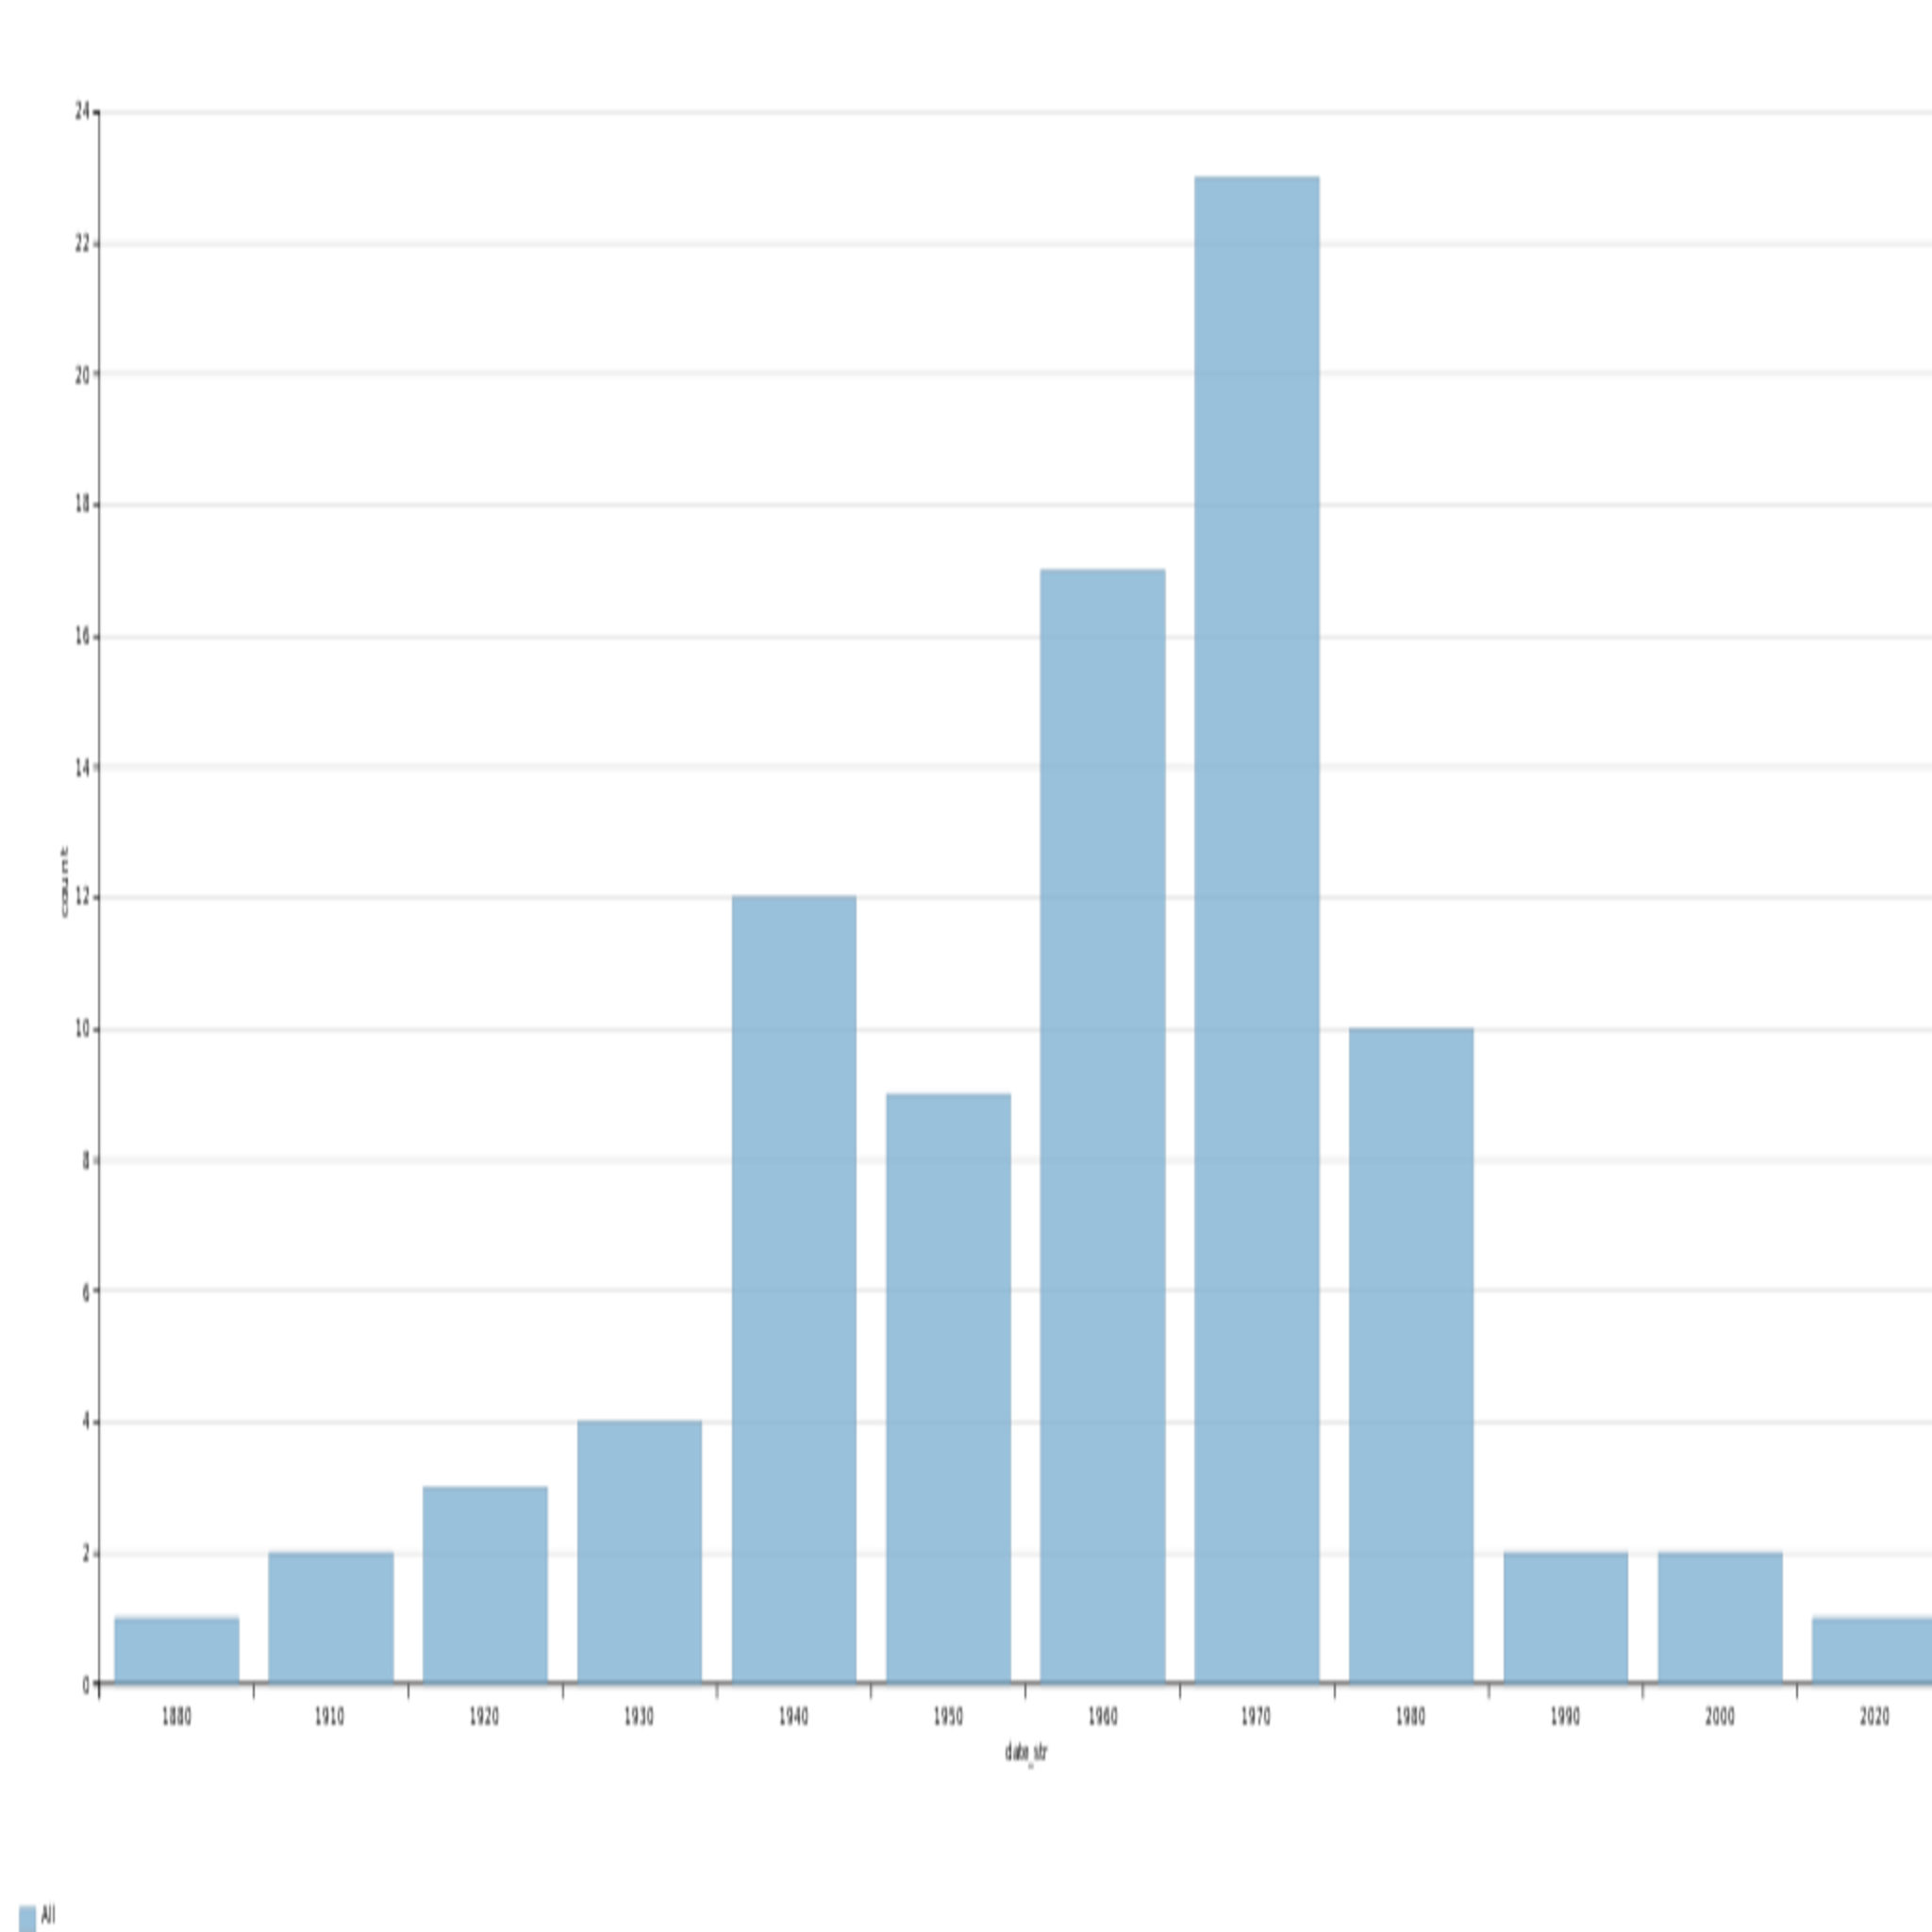
\includegraphics[width=1\textwidth]{./chapter/musical_composition/Barchart_of_The_number_of_music_compositions_in_Russia_and_USSR_every_10_years.svg.png}
	\caption[Гистограмма количества музыкальных композиций в России и СССР за каждые 10 лет с XIX века до настоящего времени]{Гистограмма количества музыкальных композиций в России и СССР за каждые 10 лет с XIX века до настоящего времени}%
\end{marginfigure}

Количество музыкальных произведений в России и СССР очень мало (97). Проанализировав несколько песен, написанных в России, таких как: <<\wdqName {Песня без слов (Кино)} {101001315}>>, <<\wdqName {Музыка нас связала} {105724079}>>, <<\wdqName {Розовое вино} {57744615}>>, не попавших в данный скрипт, стало понятно, что у этих произведений отсутствует свойство <<\wdProperty{495} {Cтрана происхождения}>>.
Далее уберём из запроса~\ref{lst:The_number_of_musical_compositions_in_Russia_for_every_10_years} строку 9 (wdt:P86 ?composer;), получим SPARQL-запрос: \href{https://w.wiki/8A8t}{https://w.wiki/8A8t}. Строка 9 ставила условие обязательного наличия композитора у музыкального произведения. Убрав эту строку, на выходе мы получаем произведения как с композиторами, так и без них. Сравним результаты обоих скриптов на диаграмме~\ref{fig:chart}. Изучив ее, можем сделать вывод, что запрос \href{https://w.wiki/8A8t}{https://w.wiki/8A8t} в основном выдаёт больше или столько же результатов, как и запрос~\ref{lst:The_number_of_musical_compositions_in_Russia_for_every_10_years}, что логично, потому что запрос \href{https://w.wiki/8A8t}{https://w.wiki/8A8t} не имеет обязательного условия наличия композитора. Но есть исключения, например: 1880-е, 1960-е. Рассмотрим, какие результаты выдают запросы за 1880 год. Запрос \href{https://w.wiki/8rd8}{https://w.wiki/8rd8} выдает 5 результатов: <<\wdqName {Всенощное бдение} {16002554}>>, <<\wdqName {String Quartet on the Theme B-la-F} {18660379}>> это произведение повторяется 4 раза. Вся проблема заключается в том, что у музыкального произведения  <<\wdqName {String Quartet on the Theme B-la-F} {18660379}>> указаны 4 композитора, поэтому оно повторяется 4 раза.

\begin{marginfigure}[0\baselineskip]
	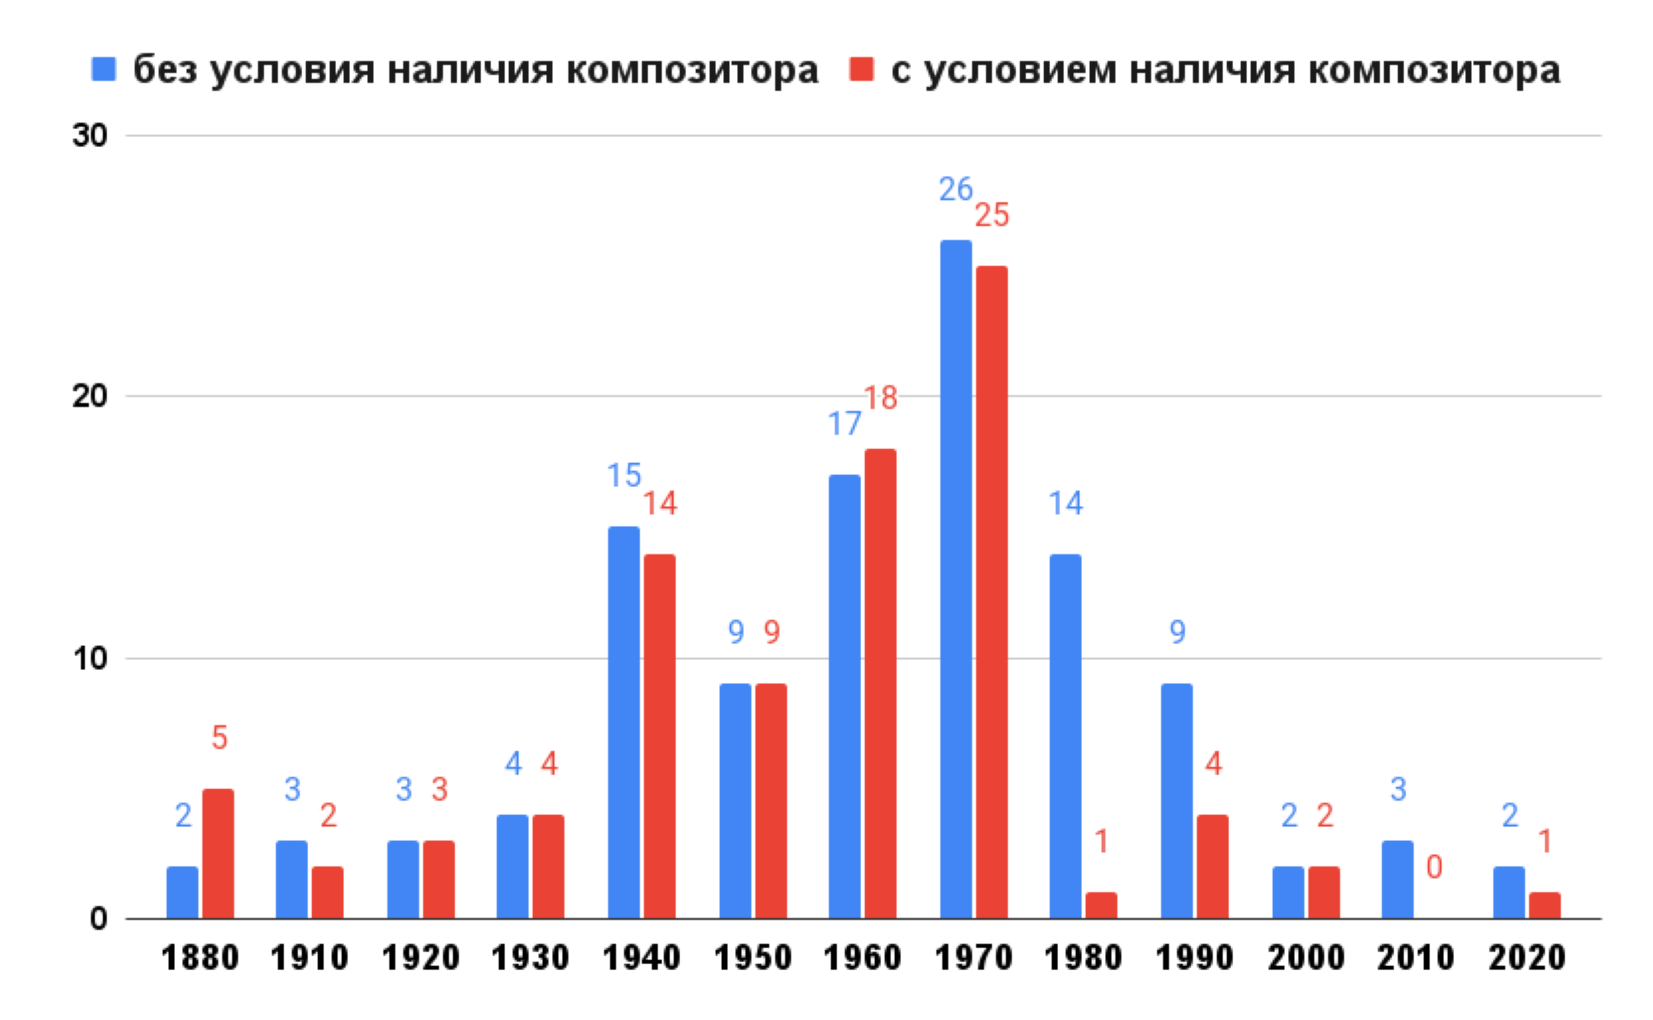
\includegraphics[width=1\textwidth]{./chapter/musical_composition/graph_of_comparison_of_readings.png}
	\caption[Диаграмма результатов запроса~\ref{lst:The_number_of_musical_compositions_in_Russia_for_every_10_years} с условием наличия композитора и без него.]{Диаграмма результатов запроса~\ref{lst:The_number_of_musical_compositions_in_Russia_for_every_10_years} с условием наличия композитора и без него.}%
	\label{fig:chart}%
\end{marginfigure}

\section{Поиск музыкальных лакун в общественном достоянии}
Задача состоит в том, чтобы найти такие музыкальные произведения, авторы которых умерли более 70 лет назад, и аудиозапись которых отсутствует на Викискладе. Найдем и упорядочим такие произведения от самых старых к новым с помощью запроса~\ref{lst:music_gaps_in_public_domain}. Существует практическая выгода и польза от~такого запроса~\ref{lst:music_gaps_in_public_domain}, поскольку видно, какие произведения можно и нужно оцифровывать (с пластинок, кассет) и загружать на Викисклад для илюстрации статей Википедии.

\begin{lstlisting}[ language=SPARQL,
                    caption={\href{https://w.wiki/88jR}{ Отсутствующие аудиозаписи музыкальных произведений, авторы которых умерли более 70 лет назад }\protect\footnotemark},
                    label=lst:music_gaps_in_public_domain,
                    texcl,
	         numbers=none
                    ]
# Search music gaps in public domain
SELECT ?composition ?compositionLabel ?publication
WHERE {
  ?composition wdt:P31 wd:Q105543609.	# instance of compostion
  ?composition wdt:P86 ?composer.		# composition has a composer
  ?composition wdt:P577 ?publication.		# composition has a publication date
  ?composer wdt:P570 ?death.			# composer has a date of death
  MINUS {?composition wdt:P51 []}.		# compositions without audio 
  FILTER(?death < "1953-01-01T00:00:00Z"^^xsd:dateTime)        # composers that passed away more than 70 years ago
  FILTER(?publication < "1953-01-01T00:00:00Z"^^xsd:dateTime)  # compositions that were published more than 70 years ago
  SERVICE wikibase:label { bd:serviceParam wikibase:language "ru,en". }
}
ORDER BY ASC(?publication)
\end{lstlisting}%
\footnotetext{Получено: \num{3771} запись на 2017 год и \num{4273} записи на 2023 год. Ссылка на SPARQL-запрос: \href{https://w.wiki/88jR}{https://w.wiki/88jR}.}

В России общественное достояние включает природные ресурсы, культурные объекты, научные достижения и образовательные ресурсы, предназначенные для общего пользования и подлежащие сохранению в соответствии с законодательством. В общем случае произведение переходит в общественное достояние в России, если с года смерти его автора прошло 70 лет. Кроме того, существует <<правило 70+4>>, согласно которому лица, трудившиеся или участвовавшие в Великой Отечественной войне, могут рассчитывать на приоритет в использовании общественных ресурсов.
\footnotetext{Ссылка на статью: \href{https://ru.wikipedia.org/?curid=31363}{https://ru.wikipedia.org/wiki/Общественное\_достояние\#Общественное\_достояние\_в\_России}.}

\section{Полнота Викиданных}
Проанализируем полноту Викиданных. Сравним количесво уникальных композиторов, предоставленных в Викиданных, с числом композиторов по другим источникам. Так же проверим, как изменяется полнота Викиданных со временем, сравнив результаты запроса~\ref{lst:BubbleChart} за~2017 год, рис.~\ref{fig:bubbleChart} и за~2022 год, рис.~\ref{fig:bubbleChart2}.

По данным \href{https://ru.wikipedia.org/wiki/Музыкальный_словарь_Гроува}{<<Музыкального словаря Гроува>>} за всю историю человечества существовало \num{20374} композиторов.

\footnotetext{\href{https://ru.wikipedia.org/wiki/Музыкальный_словарь_Гроува}{<<Музыкального словаря Гроува>>}.}

По данным категории \href{https://ru.wikipedia.org/wiki/Категория:Композиторы_по_алфавиту}{<<Композиторы по алфавиту>>} Русской Википедии существует \num{6130} композиторов.

\footnotetext{\href{https://ru.wikipedia.org/wiki/Категория:Композиторы_по_алфавиту}{<<Композиторы по алфавиту>>}.}

По данным категории \href{https://en.wikipedia.org/wiki/List_of_composers_by_name}{<<List of composers by name>>} Английской Википедии существует \num{4685} композиторов.

\footnotetext{\href{https://en.wikipedia.org/wiki/List_of_composers_by_name}{<<List of composers by name>>}.}

Количество музыкальных композиций с заполненным свойством <<\wdProperty{86}{композитор}>> равно \num{3862}, что показывает нам запрос \href{https://w.wiki/56Rc}{https://w.wiki/56Rc}, и это с учётом того, что один композитор мог написать несколько музыкальных произведений. Например, \href{https://ru.wikipedia.org/wiki/Моцарт,_Вольфганг_Амадей}{Вольфганг Амадей Моцарт} написал \num{95} произведений, что существенно снижает количество уникальных композиторов. Полученное число \num{3862}, из результатов запроса \href{https://w.wiki/56Rc}{https://w.wiki/56Rc}, меньше, чем количество композиторов из Русской и Английской Википедии и существенно меньше, чем количество композиторов из \href{https://ru.wikipedia.org/wiki/Музыкальный_словарь_Гроува}{<<Музыкального словаря Гроува>>}, что говорит нам о неполноте Викиданных.

Запрос \href{https://w.wiki/56Rj}{https://w.wiki/56Rj} по композициям с заполненным свойством <<\wdProperty{86}{композитор}>> и свойством <<\wdProperty{495}{страна происхождения}>>, имеющим значения <<\wdqName{Российская империя}{34266}>>, <<\wdqName{СССР}{15180}>> или <<\wdqName{Россия}{159}>>, выдал всего лишь \num{8} произведений, что говорит о~невозможности анализа русских музыкальных произведений в связи с недостатком данных.

Построим  две пузырьковые диаграммы композиторов с музыкальными произведениями за 2017 год, рис.~\ref{fig:bubbleChart} и за~2023 год, рис.~\ref{fig:bubbleChart2}.

\footnotetext{Получено: \num{773} записи. Ссылка на SPARQL-запрос: \href{https://w.wiki/85oS}{https://w.wiki/85oS}.}
\begin{lstlisting}[ language=SPARQL, numbers=none,
                    caption={\href{https://w.wiki/85oS}{ Пузырьковая диаграмма композиторов с музыкальными произведениями}\protect\footnotemark},
                    label=lst:BubbleChart,
                    texcl,
	         numbers=none
                    ]
# composers with musical compositions
#defaultView:BubbleChart
SELECT ?composer ?composerLabel (COUNT(*) AS ?count) WHERE {
  ?composition wdt:P31 wd:Q105543609; # this composition
               wdt:P86 ?composer.     # was written by the composer
  SERVICE wikibase:label { bd:serviceParam wikibase:language "ru, en" }
}
GROUP BY ?composer ?composerLabel
ORDER BY DESC(?count) ?composerLabel
\end{lstlisting}%

Запрос~\ref{lst:BubbleChart} выдает пузырьковую диаграмму изображенную на рис.~\ref{fig:bubbleChart} и рис.~\ref{fig:bubbleChart2}.

Размер круга означает количество написанных музыкальных композиций. Диаграмма показывает, что у одних композиторов значительно больше композиций чем у других. В~первую пятерку входят \href{https://ru.wikipedia.org/wiki/Гаде,_Нильс}{Нильс Гаде} (\num{173} композиции), \href{https://ru.wikipedia.org/wiki/Бах,_Иоганн_Себастьян}{Иоганн Себастьян Бах} (\num{155} композиций), \href{https://ru.wikipedia.org/wiki/Синдинг,_Кристиан_Август}{Кристиан Август Синдинг} (\num{125} композиций), \href{https://ru.wikipedia.org/wiki/Хальворсен,_Юхан}{Юхан Хальворсен} (\num{121} композиция), \href{https://ru.wikipedia.org/wiki/Хованесс,_Алан}{Алан Хованесс} (\num{108} композиций).

Диаграмма~\ref{fig:bubbleChart2} за 2023 год позывает, как изменилось количество написанных композиций у различный композиторов. Что бы рассмотреть подробнее, добавим в конец запроса~\ref{lst:BubbleChart} строку  \lstinline|LIMIT 12|, чтобы ограничить количество записей до 12, получим следующий запрос \href{https://w.wiki/8A2h}{https://w.wiki/8A2h}, результат на рис.~\ref{fig:bubbleChart3}. Теперь сравним результаты за~2017 год и за~2023 год.
По сравнению с 2017 годом в первую пятёрку входят \href{https://ca.wikipedia.org/wiki/Tomàs_Gil_i_Membrado}{Томас Хиль Мембрадо} (\num{1437} композиций), \href{https://ru.wikipedia.org/wiki/Гендель,_Георг_Фридрих}{Гендель Георг Фридрих} (\num{1251} композиция), \href{https://ru.wikipedia.org/wiki/Маклауд,_Кевин}{Маклауд Кевин} (\num{1237} композиций), \href{https://en.wikipedia.org/wiki/R._D._Burman}{Рахул Дев Бурман} (\num{744} композиции), \href{https://ru.wikipedia.org/wiki/Моцарт,_Вольфганг_Амадей}{Вольфганг Амадей Моцарт} (\num{703} композиции). Исходя из данных диаграмм~\ref{fig:bubbleChart} и ~\ref{fig:bubbleChart2}, можно сделать вывод, что появились новые композиторы, которые имеют значительно больше композиций. Так же можно наблюдать имена классических композиторов, например \href{https://ru.wikipedia.org/wiki/Бах,_Иоганн_Себастьян}{Иоганн Себастьян Бах} (\num{566} композиций), тоже с существенным приростом в 411 опубликованных композиций, что говорит о дополнении Викиданных ранее неучтёнными произведениями.

\begin{figure*}
	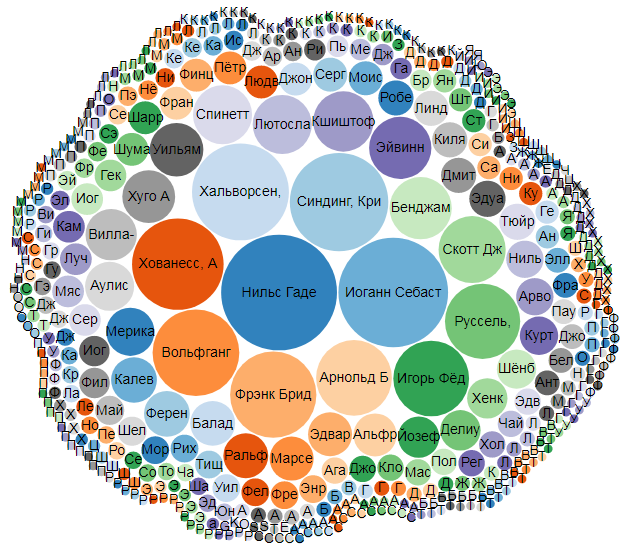
\includegraphics[width=\textwidth]{./chapter/musical_composition/Composer_of_musical_compositions_bubble_diagram.png}
	\caption[Пузырьковая диаграмма композиторов по количеству написанных композиций на~2017 год]{Пузырьковая диаграмма композиторов по количеству написанных композиций на~2017 год}%
 	\label{fig:bubbleChart}%
\end{figure*}
\begin{figure*}
	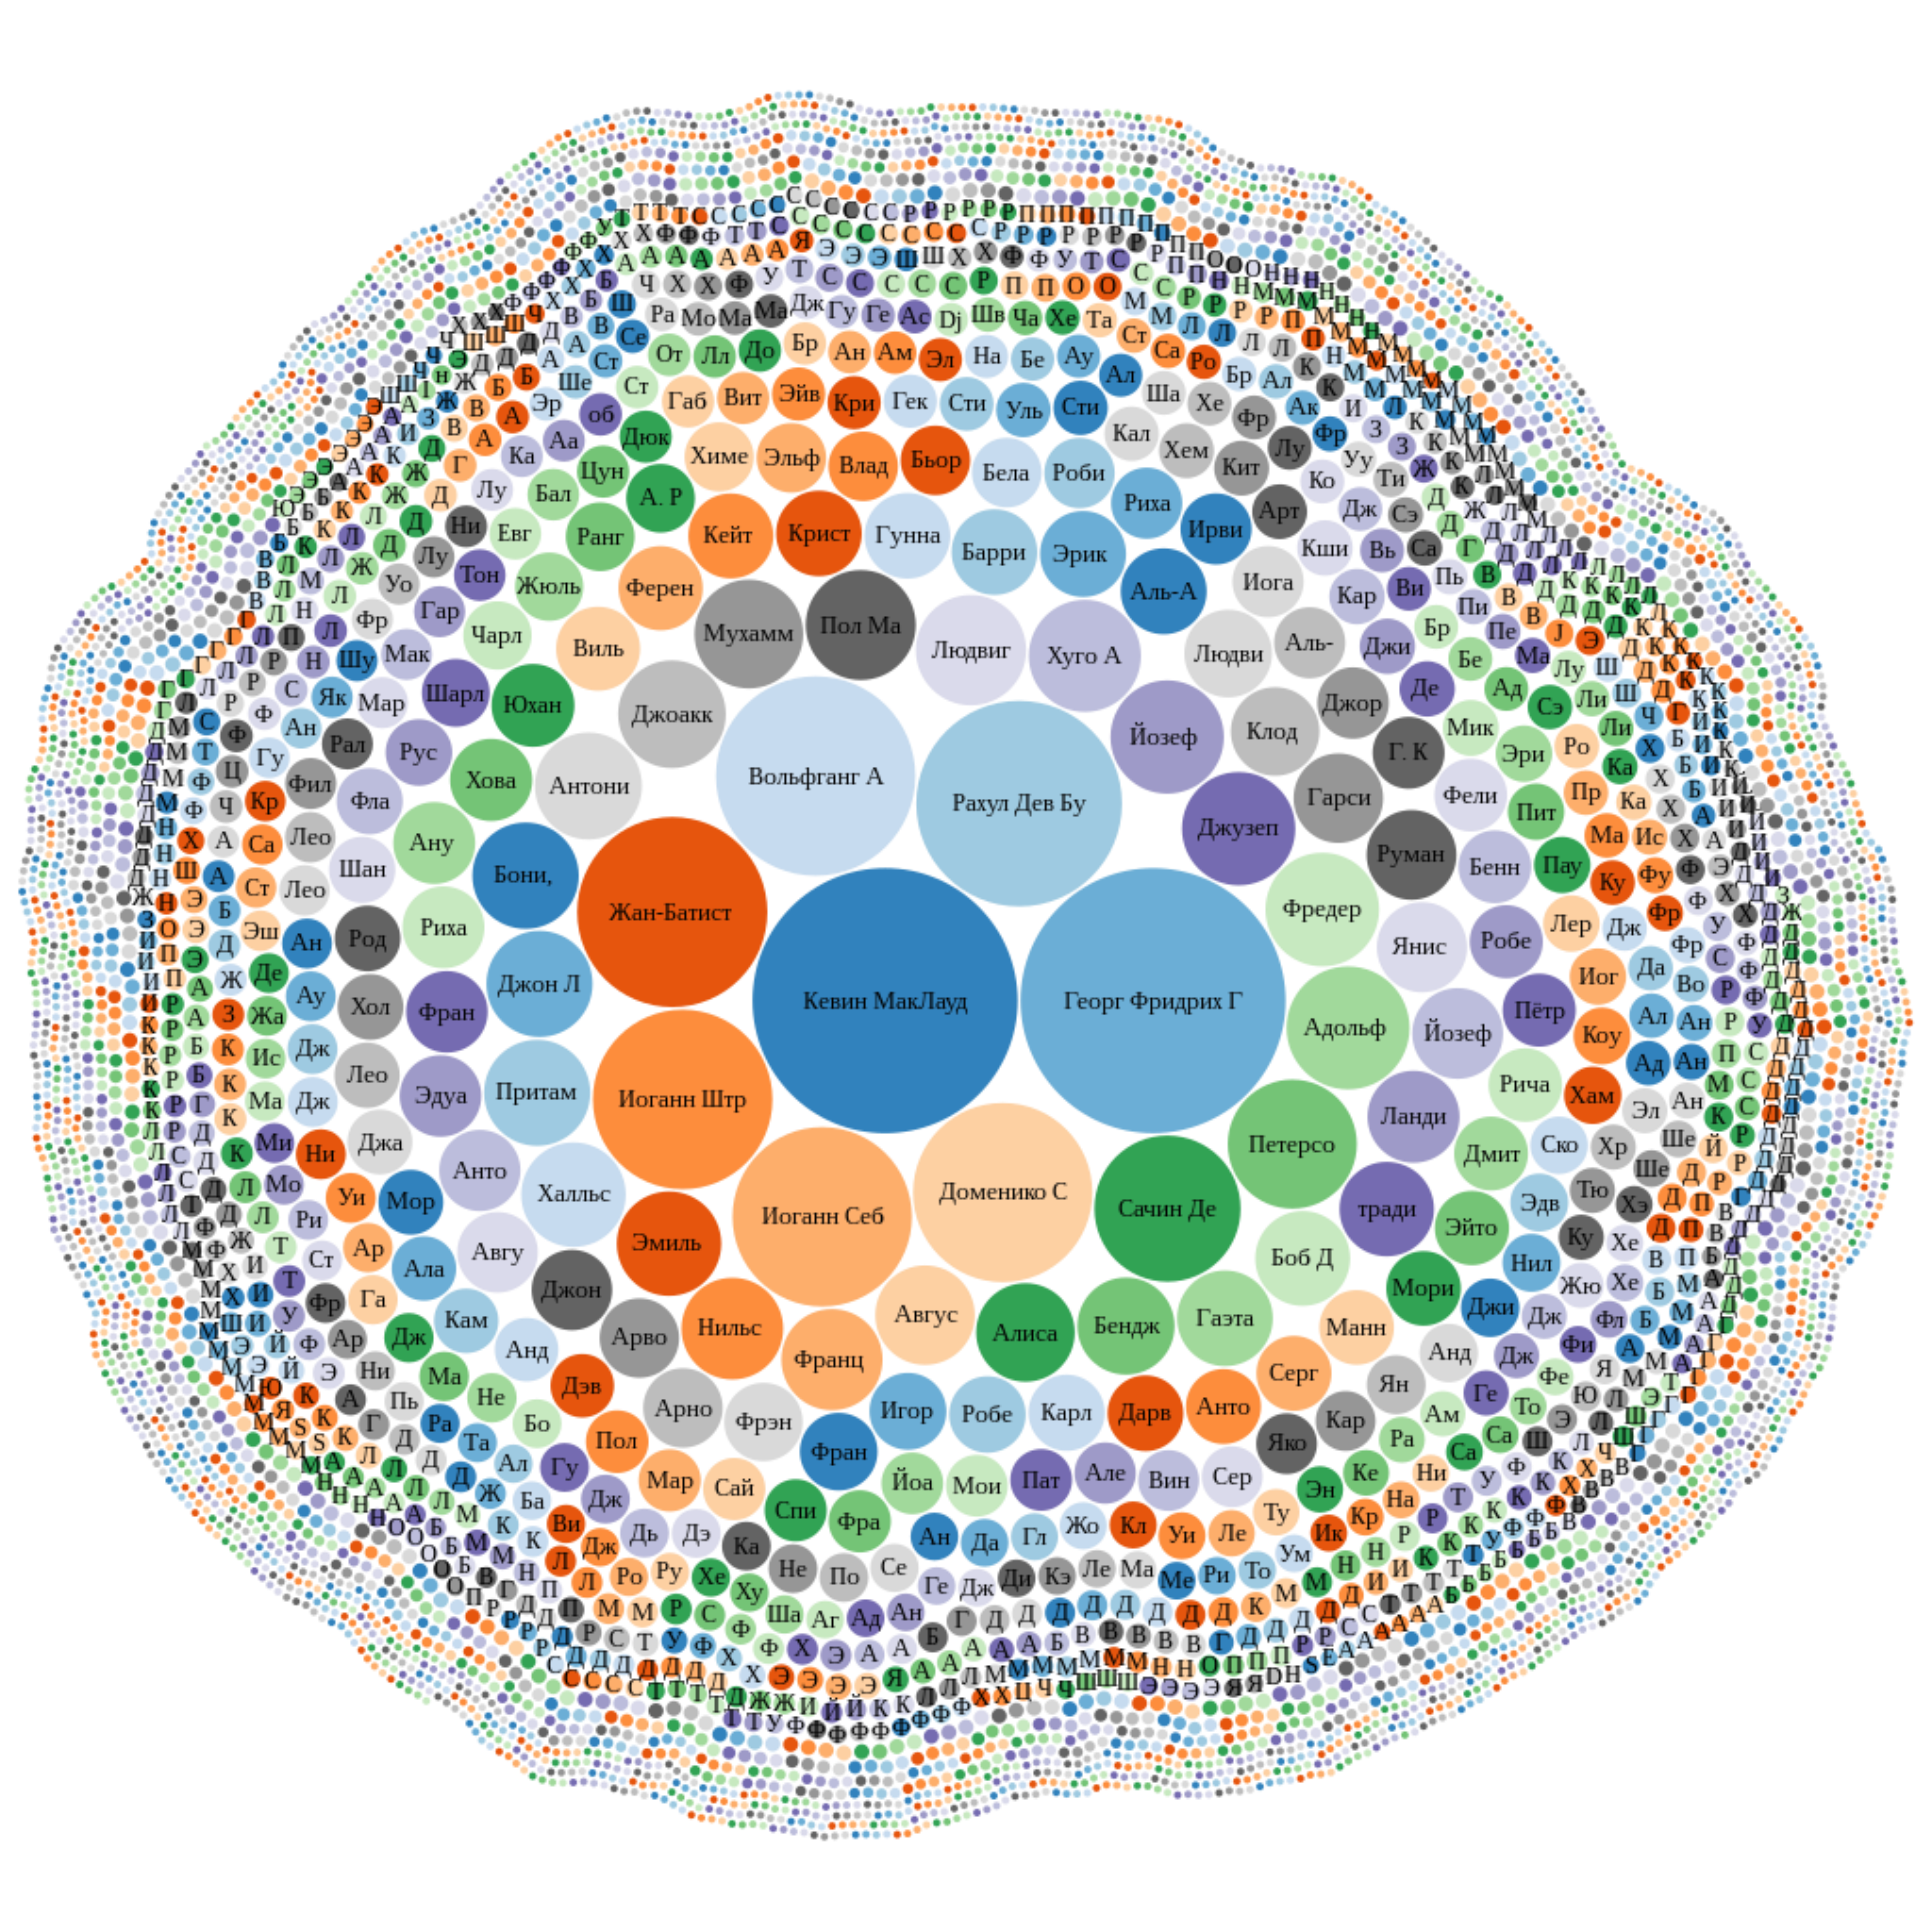
\includegraphics[width=\textwidth]{./chapter/musical_composition/Composer_of_musical_compositions_bubble_diagram.svg.png}
	\caption[Пузырьковая диаграмма композиторов по количеству написанных композиций на~2023 год]{Пузырьковая диаграмма композиторов по количеству написанных композиций на~2023 год}%
	\label{fig:bubbleChart2}%
\end{figure*}

\begin{figure*}
	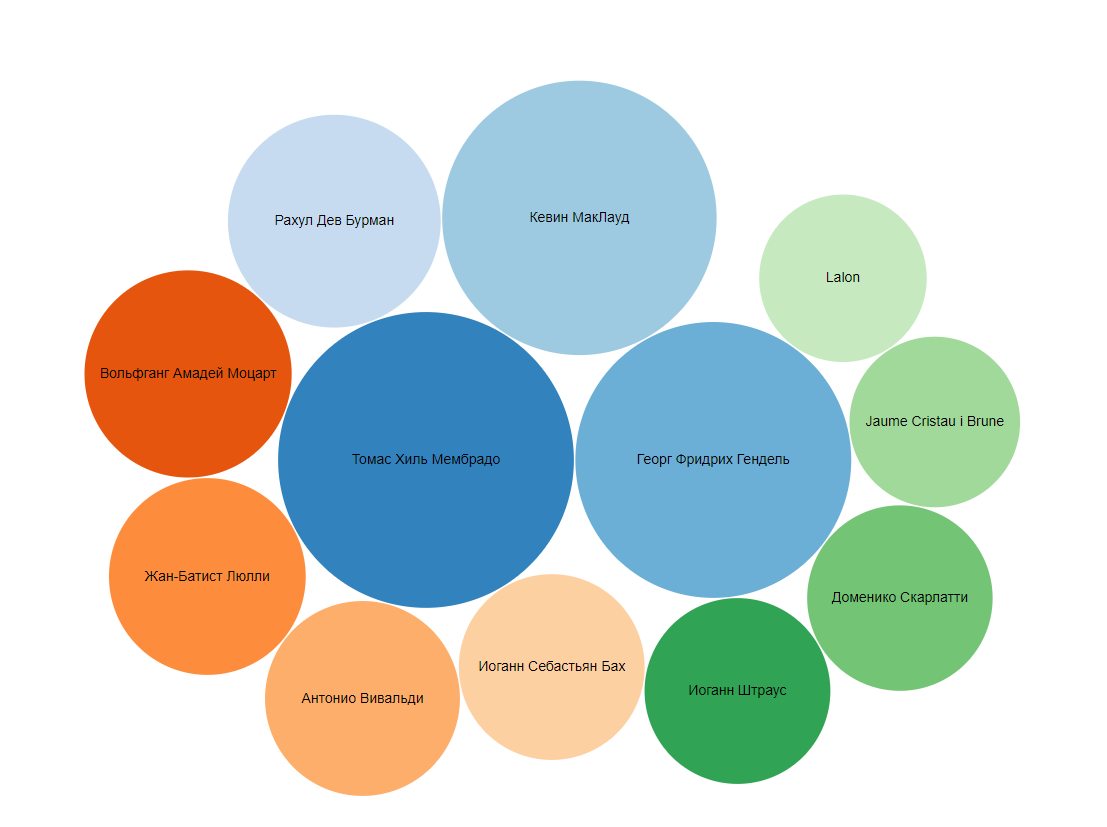
\includegraphics[width=\textwidth]{./chapter/musical_composition/Composer_of_musical_compositions_bubble_diagram.svg_2.png}
	\caption[Пузырьковая диаграмма композиторов с наибольшим количеством написанных музыкальных композиций на~2023 год]{Пузырьковая диаграмма композиторов с наибольшим количеством написанных музыкальных композиций на~2023 год}%
	\label{fig:bubbleChart3}%
\end{figure*}

\newpage

\section{Упражнения}
\begin{enumerate}
\item Найти список музыкальных композиций, созданных во время эпохи классицизма (XVII--XVIII века).
Использовать свойство: <<\wdProperty{571}{дата создания}>>.
\item Найти композитора, который написал больше симфоний, чем остальные.
Использовать свойства: <<\wdProperty{31}{экземпляр}>>, <<\wdProperty{86}{композитор}>>. Объекст: <<\wdqName {симфония} {9734}>>.
\item Построить гистограмму, на которой отображается количество музыкальных композиций группы The Beatles по году публикации.
Использовать свойства: <<\wdProperty{175}{исполнитель}>>, <<\wdProperty{577}{дата публикации}>>.

Получим следующий запрос.

\begin{lstlisting}[ language=SPARQL, numbers=none,
                    caption={\href{https://w.wiki/9Luc}{Количество музыкальных композиций The Beatles по годам издания}\protect\footnotemark},
                    label=lst:TheBeatles,
                    texcl,
	         numbers=none
                    ]
#number of musical compositions by The Beatles by year of publication
#defaultView:BarChart
SELECT  (STR(?date) AS ?date_str) (COUNT(?composition) AS ?count)  
WHERE {
  ?composition wdt:P31 wd:Q105543609; # instance of musical work
   wdt:P175 ?executor;        # composition has a executor
  wdt:P577 ?publication.      # composition has a publication date
  FILTER (?executor = wd:Q1299).  # executor = The Beatles
  BIND(YEAR(?publication) AS ?year)
  BIND(FLOOR(?year)AS ?date)
  FILTER(?publication > "1959-01-01T00:00:00Z"^^xsd:dateTime)
  FILTER(?publication < "1971-01-01T00:00:00Z"^^xsd:dateTime) 
  FILTER (!wikibase:isSomeValue(?publication)) # field "date" must be filled
}
GROUP BY ?date
\end{lstlisting}%
\footnotetext{Получено: \num{773} записи. Ссылка на SPARQL-запрос: \href{https://w.wiki/9Luc}{https://w.wiki/9Luc}.}
Запрос~\ref{lst:TheBeatles} выдает пузырьковую диаграмму изображенную на рис.~\ref{fig:ThebeatlesBubbleChart}.

В запросе~\ref{lst:TheBeatles} мы используем свойство <<\wdProperty{175}{исполнитель}>>, вместо привычного <<\wdProperty{86}{композитор}>>. Это связано с тем, что свойство <<\wdProperty{86}{композитор}>> выдает композиторов написавших музыкальное произведение, в нашем случае нужно найти музыкальные произведения исполненные группой The Beatles.

\begin{figure*}
	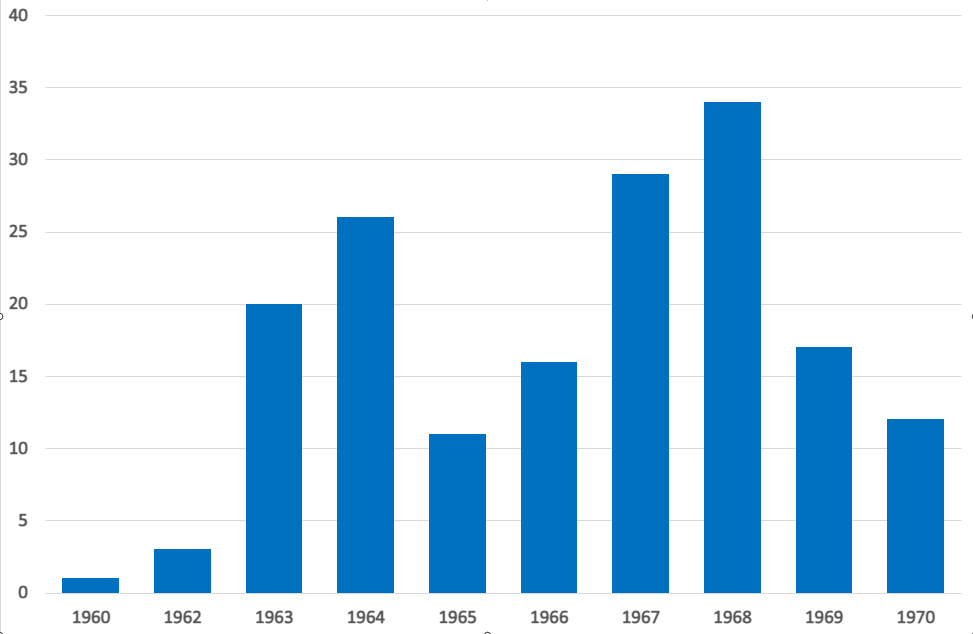
\includegraphics[width=\textwidth]{./chapter/musical_composition/BarChart_of_The_number_of_musical_comp_by The Beatles by year of publication .png}
	\caption[Гистограмма количества музыкальных композиций The Beatles по годам издания]{Гистограмма количества музыкальных композиций The Beatles по годам издания}%
 	\label{fig:ThebeatlesBubbleChart}%
\end{figure*}
\end{enumerate}
